

\section{RESULTS}
\subsubsection{Density projection upon one dimension} % (fold)
\label{ssub:density_projection_upon_one_dimension}

%\begin{figure}[htbp]
%\centering
%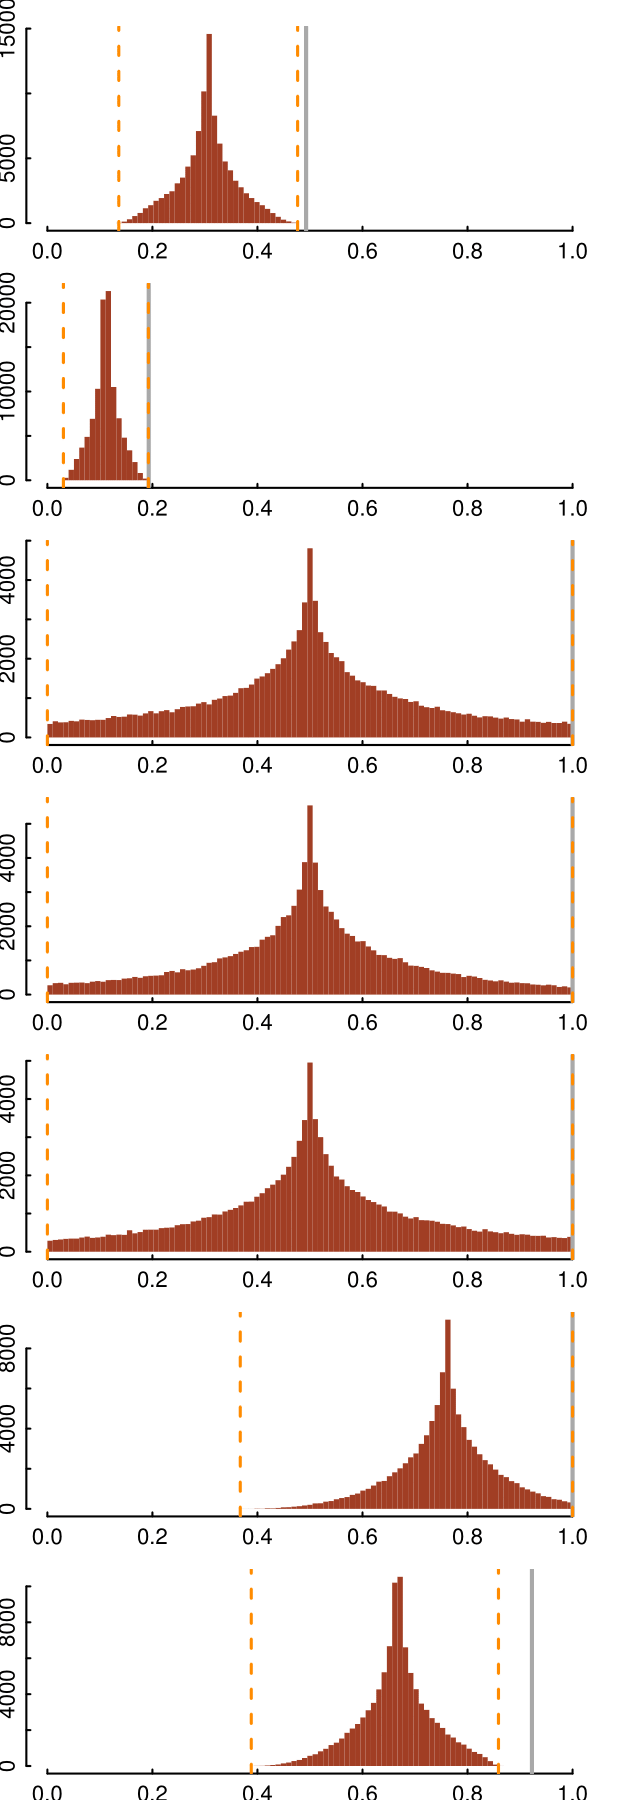
\includegraphics[width=0.5\textwidth]{sections/figs/raw_histograms.png}
%\caption{Distribution of feasible activations for [briantodo: select task percent]50\% maximal force output in the palmar direction.}
%\label{fig:raw_histograms}
%\end{figure}
Using Hit-and-Run to sample feasible activation sets, Figure \ref{fig:raw_histograms} shows the distributions of activation solutions for a palmar submaximal force resulting from [briantodo number] solutions computed with Hit-and-Run sampling. This is the first time (to our knowledge) that the internal structure of the feasible activation set has been visualized for a sub-maximal force.
Notice also that the lower and upper bounds of the activations (i.e., the dashed lines that indicate their bounding box), are uniquely uninformative of the actual density of distribution of feasible activations. Note also that the activation needed for the maximal force output (thick gray line) is very often not the mode of the activations at [briantodo select correct number]50\%[maytodo: can we set this as a variable and use throughout?] of output.
\\
This figure shows ... [briantodo]
talk about what the bounds mean with respect to the upper and lower bounds.
Talk about the function of each muscle, with respect to the moment arm matrix and the relevant cell of the A matrix.
% subsubsection density_projection_upon_one_dimension (end)


\subsection{Activation spaces for increasing force} % (fold)
\label{sub:activation_spaces_for_increasing_force}

[1. briantodo generate pdfs as separate pages][2maytodo: insert a single pdf for palmar direction, and add other pages to the appendix]
[briantodo write about how they are skewed, constrained, etc. Produce stats for each of the histograms and superimpose the data temporarily so you can write about it]

\begin{figure}[htbp]
\centering
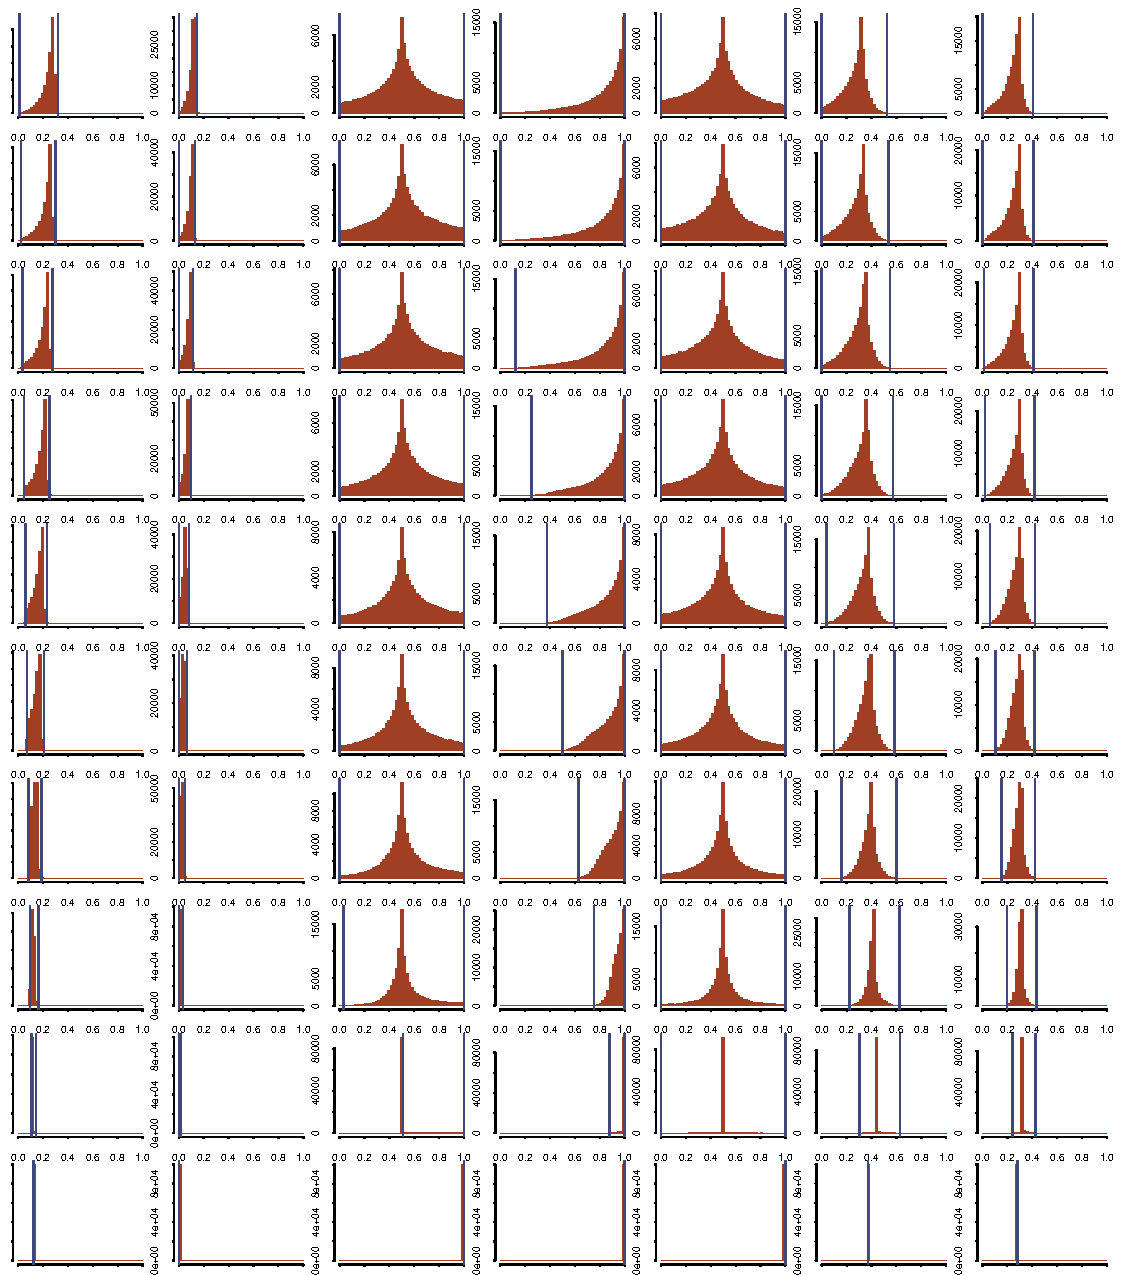
\includegraphics[width=\textwidth]{figs/XY_alphaProgression.pdf}
\caption{Distribution of activations in $XY$-direction and changing force}
\label{fig:XY_progression}
\end{figure}
% subsection activation_spaces_for_increasing_force (end)

\subsection{Parallel Coordinates} % (fold)
\label{sub:parallel_coordinates}
briantodo: add the following figures:
\begin{itemize}
	\item{parcoord Full}
	\item{parcoord muscle limited to 75\%, then 50\%, then 25\% of its normalized maximal activation}
	\item{parcoord cost limited to 25\% of costfn1, costfn2, costfn3}
\end{itemize}

discuss what happens when you bring each of those muscles down, using the R produced stats.
talk about how when you add X as a constraint, most of the solutions are distributed across the other muscles between X and X. Say which ones go up, which go down- which ones become clustered and which ones lose their peak/spike.

% subsection parallel_coordinates (end)